\documentclass[letterpaper]{article}
\usepackage[T1]{fontenc}
\usepackage{newtxtext}
\usepackage{newtxmath}
\usepackage[margin=0.85in]{geometry}
\usepackage[hyphens]{url}
\urlstyle{rm}
\def\UrlFont{\rm}
\usepackage{natbib}
\usepackage{booktabs}
\usepackage{amsmath}
\usepackage{amssymb}
\usepackage{amsthm}
\usepackage{array}
\usepackage{graphicx}
\usepackage{multirow}
\usepackage{float}
\usepackage{placeins}
\frenchspacing

\setcounter{secnumdepth}{2}
\newtheorem{proposition}{Proposition}

\title{MESANet: Affine-Anchored Dual-Coordinate Forecasting for Wearable Irregular Time Series}
\author{Anonymous Submission}
\date{}

\begin{document}
\maketitle

\begin{abstract}
Wearable irregular time series vary simultaneously in sensor value scale,
observation support, and within-patch waveform. Pooling these factors into one
patch token can preserve local level while erasing ordered motion, or preserve
motion while mixing unsupported temporal ranges. We introduce the
Multiresolution Evidence Separation and Anchoring Network (MESANet), an
end-to-end forecasting backbone that represents every variable through two
complementary coordinates. A masked affine anchor canonicalizes each observed
history and restores its physical coordinate after prediction. A
multiresolution support branch forms a bounded low-frequency coordinate, while an
ordered waveform branch encodes masked values, observation patterns, and first
differences without pooling away patch order. The coordinates produce a
low-rank cosine forecast and a direct trajectory; fixed low-frequency
subtraction with coefficient $\rho=0.5$ bounds overlap before summation. The analysis
characterizes conditional affine equivariance, collisions induced by pooled
patch statistics, and dual-coordinate excess risk through low-frequency
approximation, waveform residual, and subspace overlap. On six wearable
datasets, one public comparator per dataset is frozen by validation error
before five-run test evaluation. MESANet obtains lower mean error in 9 of 12
mean squared error (MSE) and mean absolute error (MAE) cells and on both metrics
for four datasets; six cells have paired bootstrap intervals over optimization
runs favoring MESANet. Parameter-matched controls
support the dual-coordinate factorization, multiresolution support, and ordered
discrete cosine transform (DCT) basis, while showing that waveform and
affine-anchor contributions are regime dependent. HumanActivity MSE and
USC-HAD delimit the empirical scope.
\end{abstract}

\section{Introduction}

Irregular multivariate time-series (IMTS) forecasting predicts future values
from asynchronous and partially observed histories. Continuous-time dynamics,
time-aware attention, graph propagation, and adaptive patching make timestamps
and missingness visible to the predictor~\citep{rubanova2019latent,
shukla2021mtan,cru2022,raindrop2022,grafiti2024,tpatchgnn2024,apn2026,
kafnet2026}. Wearable streams add structured variation: sensor offsets and
amplitudes change across users and sessions, sensor groups are not always
co-observed, and short motion transients coexist with slower postural trends.
An effective wearable forecaster must therefore preserve the physical sensor
coordinate, observation support, and ordered waveform simultaneously.

Patch forecasting compresses observations into a finite set of tokens, but one
token is often asked to perform incompatible roles. A wider or adaptively
selected support can stabilize a sparse patch, yet averaging that support can
erase within-patch order. Conversely, a short ordered patch preserves motion
but may lack enough evidence under stale or asynchronous sampling. Figure
\ref{fig:mesa-motivation} illustrates the support side of this conflict: the
predictive temporal range changes across local observation states, so neither
one selected range nor unconditional scale mixing is uniformly reliable. The
same compression can also create waveform collisions: increasing and decreasing
segments can share their mean, variance, density, and endpoints after pooling
while implying different futures.

\begin{figure}[t]
\centering
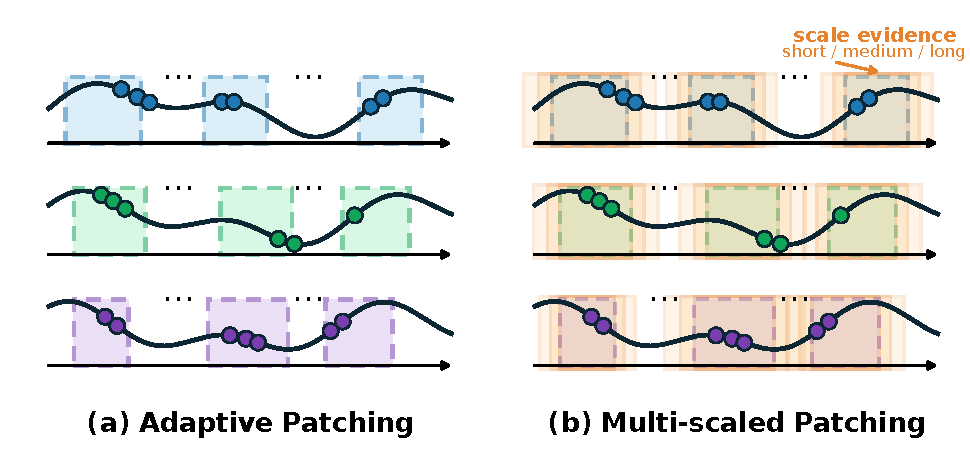
\includegraphics[width=\columnwidth]{figures/final/mesa_fig1_apn_like_v540.pdf}
\caption{Single-support adaptive patching and multiscale patch evidence.
Irregular density and recency change the useful temporal range; pooling any
selected range can additionally suppress ordered within-patch motion.}
\label{fig:mesa-motivation}
\end{figure}

This observation suggests a representation principle: support-scale evidence
and ordered waveform evidence should be retained as distinct forecast
coordinates. The first coordinate needs a stable value anchor and alternative
causal supports; the second needs the original order of masked observations
and local differences. Their forecasts should be combined without allowing
the waveform path to duplicate the low-frequency component without control.
This forecast-space factorization, rather than any individual encoder
primitive, is the central design: evidence remains coordinate-specific until
the final prediction geometry is formed.

We instantiate the principle in the \emph{Multiresolution Evidence Separation
and Anchoring Network} (MESANet), shown in Figure~\ref{fig:v665-framework}.
Masked affine anchoring first maps each sample--variable history to a canonical
coordinate. The low-frequency branch combines a fixed patch token with a bank
of causal support tokens through bounded scale admission. In parallel, the
waveform branch embeds ordered normalized values, masks, and first differences.
The two branches retain coordinate-specific variable representations. A
discrete cosine transform (DCT) head predicts a compact level trajectory,
whereas a direct head
predicts the waveform trajectory. Before addition, fixed subtraction with
$\rho=0.5$ attenuates the direct head's low-frequency component. Finally,
the stored affine coordinate restores the sensor scale.

The representation has three structural properties. Reversible anchoring makes
the complete forecast conditionally equivariant to positive sample-variable
affine transformations. Retaining ordered fields and support state refines a
fixed summary and can reduce collision risk when the refinements change the
conditional future. For the separation operator, an exact risk decomposition
identifies low-coordinate error, waveform residual error, and subspace overlap.
These properties motivate the operator and specify when its two coordinates can
help; they are not a universal learning guarantee.

We evaluate the complete backbone under a shared protocol on six public
wearable datasets. For each dataset, validation MSE with a validation-MAE
tie-break freezes one public comparator, which is then used for both test
metrics. Five-run comparisons favor MESANet in mean error for 9 of 12 metric
cells and on both MSE and MAE for MHEALTH, OPPORTUNITY, PAMAP2, and REALDISP;
six cells have paired bootstrap intervals over optimization runs favoring
MESANet. Its
HumanActivity MAE improves while MSE is slightly worse, and PatchTST remains
better on USC-HAD. These boundaries show where a compact regular patch model
already matches the subject partition.

Our contributions are:
\begin{itemize}
  \item We identify a potential dual representation failure in wearable IMTS
  patches: compression can discard distinctions in temporal support or
  waveform order that are predictive in some, but not all, evaluated datasets.
  \item We introduce MESANet, a new end-to-end backbone that realizes this
  factorization through masked affine anchoring, bounded multiresolution
  support tokens, ordered waveform tokens, and fixed DCT-subspace separation.
  \item We provide a design analysis connecting low-frequency approximation,
  waveform residual prediction, and subspace overlap, together with structural
  affine-equivariance and collision results.
  \item Validation-frozen five-run comparisons, three-run final-model controls,
  parameter sensitivity, efficiency profiling, and a 24-subject strict
  leave-one-subject-out (LOSO)
  stress test characterize predictive accuracy, component contributions,
  parameter behavior, computational cost, and subject-transfer boundaries.
\end{itemize}

\section{Related Work}

\textbf{Irregular time-series forecasting.}
Recurrent imputation and decay models handle missing observations explicitly
\citep{che2018grud,cao2018brits}; latent ordinary differential equations
(ODEs), neural controlled differential equations, continuous recurrent units,
and time-aware attention instead model
continuous-time evolution~\citep{rubanova2019latent,kidger2020neuralcde,
shukla2021mtan,cru2022}. Raindrop and GraFITi use graph structure to transfer
information across variables or observations~\citep{raindrop2022,grafiti2024}.
These models establish timestamps, masks, and variable dependency as central
IMTS inputs. MESANet focuses on the earlier representation step: preserving
support and ordered motion as complementary patch coordinates before their
forecasts are combined.

\textbf{Patch and multiscale forecasting.}
PatchTST, TimesNet, iTransformer, TimeMixer, and Pathformer show that patch
tokens and multiscale pathways are effective on regular series
\citep{nie2023patchtst,timesnet2023,liu2024itransformer,timemixer2024,
pathformer2024}. For IMTS, tPatchGNN learns transformable patches, APN learns
adaptive patch aggregation, and KAFNet introduces canonical alignment
\citep{tpatchgnn2024,apn2026,kafnet2026}. MESANet differs by maintaining a
bounded support-derived level coordinate and an ordered waveform coordinate
until forecast formation, then controlling their overlap in the forecast
domain. The public comparison therefore includes these direct patch
families together with GraFITi and PatchTST.

\textbf{Wearable representation and normalization.}
Wearable models commonly exploit local motion and cross-sensor structure for
activity recognition~\citep{ordonez2016deepconv,abedin2021attend,
zhou2022tinyhar}; our target is continuous future sensor values and does not
use activity or subject labels. Reversible instance normalization (RevIN)
demonstrates the value of reversible instance coordinates under distribution
shift~\citep{kim2022revin}. MESANet
extends the reversible principle to masked sample--variable histories and
couples it with irregular support and waveform coordinates inside a forecasting
backbone.

\section{Methodology}
\label{sec:method}

\subsection{Problem Setting and Overview}

Let $X=\{(t_j,\mathbf{x}_j,\mathbf{m}_j)\}_{j=1}^{L}$ be an
irregular multivariate history. Index $j$ denotes a history event on the union
of observed timestamps, $\mathbf{x}_j\in\mathbb{R}^{D}$ stores the sensor
values at that event, and $\mathbf{m}_j\in\{0,1\}^{D}$ indicates which values
are observed. Given future query times $\{t_h^+\}_{h=1}^{H}$, the model
predicts $\widehat{\mathbf y}_h\in\mathbb{R}^{D}$. Future availability masks
are used only by the loss and evaluator.

Figure~\ref{fig:v665-framework} gives the complete forward path. MESANet first
canonicalizes each sample--variable history using observed entries. It then
builds two patch sequences: a low-frequency coordinate $\mathbf L$ retaining
fixed and multiresolution support evidence, and an ordered waveform coordinate
$\mathbf W$ retaining within-patch values, masks, and first differences.
Coordinate-specific representations produce low- and high-frequency forecasts.
A bounded projection controls their subspace overlap before affine restoration.

\begin{figure*}[t]
\centering
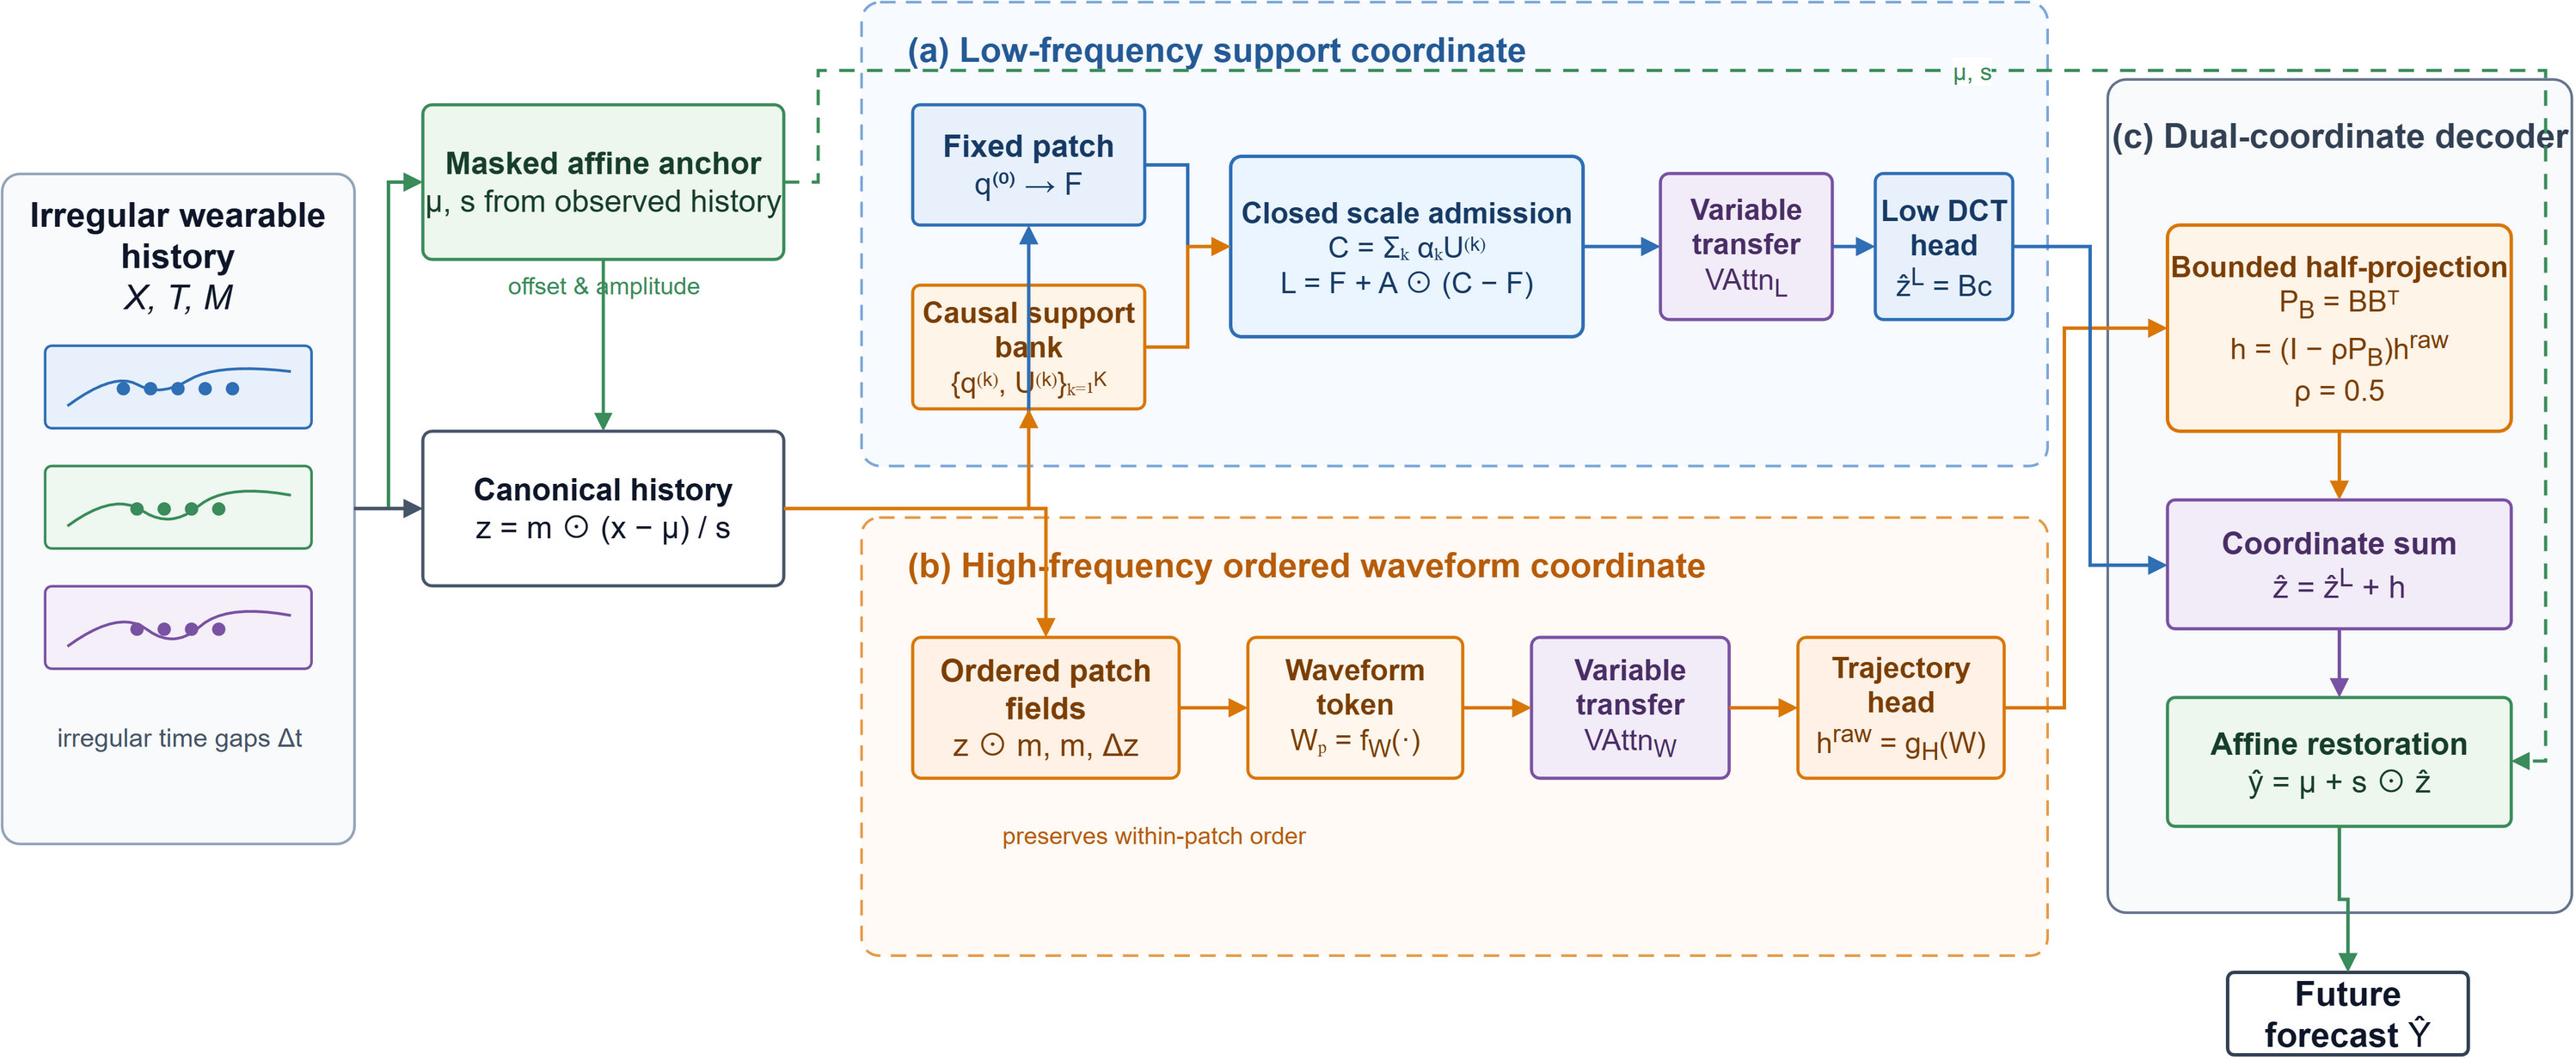
\includegraphics[width=\textwidth]{figures/final/mesa_fig2_v676.png}
\caption{MESANet architecture. Masked affine anchoring feeds a low-frequency
support coordinate and an ordered waveform coordinate. Coordinate-specific
variable transfer and forecast heads are combined by bounded DCT-subspace
separation before affine restoration.}
\label{fig:v665-framework}
\end{figure*}

\subsection{Masked Affine Anchoring}

For sample $b$ and variable $i$, the number of observed history values, their
mean, and their scale are
\begin{align}
n_{bi} &= \sum_{j=1}^{L}m_{bji}, \label{eq:count}\\
\mu_{bi} &= \frac{\sum_jm_{bji}x_{bji}}{\max(n_{bi},1)}, \label{eq:mean}\\
s_{bi} &= \max\!\left(
\sqrt{\frac{\sum_jm_{bji}(x_{bji}-\mu_{bi})^2}{\max(n_{bi},1)}+\epsilon},
s_{\min}\right). \label{eq:scale}
\end{align}
When $n_{bi}=0$, we use $(\mu_{bi},s_{bi})=(0,1)$. The canonical history is
\begin{equation}
z_{bji}=m_{bji}\frac{x_{bji}-\mu_{bi}}{s_{bi}},
\label{eq:canonical}
\end{equation}
and the final normalized forecast $\widehat z_{bhi}$ is restored by
\begin{equation}
\widehat y_{bhi}=\mu_{bi}+s_{bi}\widehat z_{bhi}.
\label{eq:restore}
\end{equation}
The anchor keeps offset and amplitude outside the learned dynamics while masks
prevent unobserved placeholders from entering its statistics.

\subsection{Low-Frequency Support Coordinate}

Let $\tau_p$ be the right boundary of patch $p$ and $I_p$ its fixed causal
interval. The fixed branch summarizes observed canonical values in $I_p$ using
density, nonempty support, mean, variance, first and last values, local slope,
observed span, recency, and the patch center. We denote this history-only
statistic by $\mathbf q^{(0)}_{bip}$. A fixed encoder with patch-time and
variable embeddings forms
\begin{equation}
\mathbf F_{bip}=f_F\!\left(
[\mathbf q^{(0)}_{bip},\operatorname{TE}(\tau_p),\mathbf e_i]\right).
\label{eq:fixed-token}
\end{equation}
Here, $\operatorname{TE}(\tau_p)$ is the patch-time embedding, $\mathbf e_i$
is the learned variable embedding, and $f_F$ is the fixed-coordinate encoder.

In parallel, $K$ causal exponential supports retain alternative ranges. For a
learnable positive width $w_k$, observation $j$ receives
\begin{align}
r^{(k)}_{bipj} &=m_{bji}\mathbf 1[t_j\leq\tau_p]
\exp\!\left(-\frac{\tau_p-t_j}{w_k+\epsilon}\right), \label{eq:support-weight}\\
\omega^{(k)}_{bipj} &=
\frac{r^{(k)}_{bipj}}{\sum_{\ell}r^{(k)}_{bip\ell}+\epsilon}.
\label{eq:normalized-weight}
\end{align}
The same statistic fields are recomputed with $\omega^{(k)}$, producing
$\mathbf q^{(k)}_{bip}$ and token $\mathbf U^{(k)}_{bip}$. Thus every support
describes the same variable and anchor but uses a different causal range. A
history-state score selects their mixture:
\begin{align}
\ell^{(k)}_{bip} &= f_\alpha(\mathbf q^{(k)}_{bip},\tau_p,\mathbf e_i)
+ b_k(\mathbf q^{(0)}_{bip}), \label{eq:scale-logit}\\
\alpha^{(k)}_{bip} &=
\frac{\exp(\ell^{(k)}_{bip})}{\sum_{r=1}^{K}\exp(\ell^{(r)}_{bip})},
\label{eq:scale-softmax}\\
\mathbf C_{bip} &= \operatorname{LN}\!\left(
\sum_{k=1}^{K}\alpha^{(k)}_{bip}\mathbf U^{(k)}_{bip}+\mathbf e_i\right).
\label{eq:scale-token}
\end{align}
Here and below, $\operatorname{LN}$ denotes layer normalization.

A bounded vector-valued admission map uses the fixed and scale statistics and tokens:
\begin{align}
\mathbf A_{bip} &= \sigma\!\left(f_A(\mathbf F_{bip},\mathbf C_{bip},
\mathbf q^{(0)}_{bip},\textstyle\sum_k\alpha^{(k)}_{bip}\mathbf q^{(k)}_{bip})
\right), \label{eq:admission}\\
\mathbf L_{bip} &= \operatorname{LN}\!\left(
\mathbf F_{bip}+\mathbf A_{bip}\odot(\mathbf C_{bip}-\mathbf F_{bip})\right).
\label{eq:level-token}
\end{align}
Since $\mathbf A_{bip}\in(0,1)^d$, each pre-normalization dimension lies
between its fixed and multiresolution values. The low-frequency branch can
therefore admit longer support without an unrestricted additive correction.

\subsection{Ordered Waveform Coordinate}

Summary statistics in Eq.~\eqref{eq:fixed-token} intentionally suppress
within-patch order. MESANet preserves that order in a separate field. For the
$P$ positions assigned to patch $p$, let $\mathbf z_{bip}\in\mathbb R^P$ and
$\mathbf m_{bip}\in\{0,1\}^{P}$ be the canonical values and masks. The masked
first difference is
\begin{equation}
\begin{aligned}
\Delta\mathbf z_{bip}[r] ={}&
\mathbf m_{bip}[r]\mathbf m_{bip}[r-1] \\
&\cdot(\mathbf z_{bip}[r]-\mathbf z_{bip}[r-1]),\quad r>1,
\end{aligned}
\label{eq:wave-diff}
\end{equation}
with zero at $r=1$. The ordered waveform token is
\begin{equation}
\mathbf W_{bip}=f_W\!\left(
[\mathbf z_{bip}\odot\mathbf m_{bip},\mathbf m_{bip},
\Delta\mathbf z_{bip},\mathbf e_i]\right).
\label{eq:wave-token}
\end{equation}
Unlike $\mathbf q^{(k)}$, this vector is sensitive to the ordering of observed
motion inside a patch. Masks distinguish an actual zero from an unavailable
position, while first differences expose local velocity without replacing the
level coordinate.

\subsection{Dual-Coordinate Forecasting}

MESANet retains separate support and waveform representations through variable
interaction. In the default implementation, scaled dot-product attention is
applied to each coordinate at every patch:
\begin{align}
\widetilde{\mathbf L}_{bp} &=
\operatorname{VAttn}_L(\mathbf L_{bp}), \label{eq:level-transfer}\\
\widetilde{\mathbf W}_{bp} &=
\operatorname{VAttn}_W(\mathbf W_{bp}). \label{eq:wave-transfer}
\end{align}
The operators $\operatorname{VAttn}_L$ and $\operatorname{VAttn}_W$ are
scaled dot-product attention across variables for the support and waveform
coordinates, respectively.
This coordinate-specific parameterization preserves the branch identities.
The factorization concerns the representations and forecast geometry, not a
requirement that their transfer parameters be disjoint; Section~\ref{sec:ablation}
therefore includes an equal-capacity shared-transfer control.

Let $\mathbf B\in\mathbb R^{H\times R}$ contain the first $R$ orthonormal
discrete-cosine basis vectors, where $R\ll H$. A low head maps the ordered
level-token trajectory to coefficients $\mathbf c_{bi}\in\mathbb R^R$:
\begin{align}
\mathbf c_{bi} &= g_L(\operatorname{vec}\{\widetilde{\mathbf L}_{bip}\}_{p=1}^{P}),
\label{eq:low-coeff}\\
\widehat{\mathbf z}^{L}_{bi} &= \mathbf B\mathbf c_{bi}.
\label{eq:low-forecast}
\end{align}
The waveform head directly predicts an $H$-step trajectory
\begin{equation}
\mathbf h^{\rm raw}_{bi}=g_H(
\operatorname{vec}\{\widetilde{\mathbf W}_{bip}\}_{p=1}^{P}).
\label{eq:raw-high}
\end{equation}
To avoid both unconstrained duplication and exact orthogonality, MESANet uses
the fixed bounded separation strength $\rho=1/2$ and applies
\begin{align}
\mathbf P_B &= \mathbf B\mathbf B^\top, \label{eq:projector}\\
\mathbf h_{bi} &= (\mathbf I-\rho\mathbf P_B)\mathbf h^{\rm raw}_{bi},
\label{eq:soft-separation}\\
\widehat{\mathbf z}_{bi} &= \widehat{\mathbf z}^{L}_{bi}+\mathbf h_{bi}.
\label{eq:coordinate-sum}
\end{align}
Equations~\eqref{eq:restore} and \eqref{eq:coordinate-sum} complete the
end-to-end forecast. We train all modules jointly with
\begin{equation}
\mathcal L=\operatorname{MSE}_{m_y}(\widehat Y,Y)
+\lambda_{\rm MAE}\operatorname{MAE}_{m_y}(\widehat Y,Y),
\label{eq:loss}
\end{equation}
where $m_y$ contains only target availability. Here MSE and MAE denote masked
mean squared error and mean absolute error, respectively.

\subsection{Design Analysis}

The first two propositions record structural consequences of anchoring and
representation refinement. The third directly analyzes the bounded forecast
operator. Together they motivate the architecture and identify conditions for
improvement rather than assert a dataset-independent advantage.

\textbf{Proposition 1 (conditional affine equivariance).}
For a nonempty sample--variable history, inactive scale floor, and
$\epsilon=0$, transform observed and future values by $x'=ax+c$ and $y'=ay+c$
with $a>0$. For fixed model parameters, MESANet satisfies
$\widehat y'=a\widehat y+c$.

The canonical history, masks, support tokens, waveform tokens, and normalized
forecast are unchanged; only $(\mu,s)$ becomes $(a\mu+c,as)$. The supplement
gives the proof and the finite-$\epsilon$ departure.

\textbf{Proposition 2 (patch-statistic collision).}
Let $Q=\phi(X)$ be a fixed pooled patch statistic. Suppose a conditional slice
$Q=q$ contains two ordered/support states $S=s_1,s_2$ with probabilities
$\pi$ and $1-\pi$, and conditional future means $\boldsymbol\mu_1\neq
\boldsymbol\mu_2$. Under squared loss, the Bayes-risk gap between a
$Q$-measurable predictor and an $(Q,S)$-measurable predictor is
\begin{equation}
\mathcal R_Q^*(q)-\mathcal R_{Q,S}^*(q)
=\pi(1-\pi)\|\boldsymbol\mu_1-\boldsymbol\mu_2\|_2^2.
\label{eq:collision}
\end{equation}
Thus distinct waveforms or support states collapsed by the same statistic
create irreducible error. MESANet makes both refinements available; the result
does not assert that they are informative on every dataset.

\textbf{Proposition 3 (dual-coordinate risk decomposition).}
Let $\boldsymbol\mu(X)=\mathbb E[\mathbf Z^+\mid X]$ be the conditional mean
of the normalized future, let $\boldsymbol\ell(X)\in\operatorname{span}(B)$
be the low-coordinate forecast, and let $\mathbf r(X)$ be the raw waveform
forecast. For
$\mathbf f_\rho=\boldsymbol\ell+(I-\rho P_B)\mathbf r$, its excess squared
risk over the Bayes predictor decomposes exactly as
\begin{align}
\mathcal R(\mathbf f_\rho)-\mathcal R^*
={}&\mathbb E\|P_B\boldsymbol\mu-\boldsymbol\ell
 -(1-\rho)P_B\mathbf r\|_2^2 \nonumber\\
&+\mathbb E\|(I-P_B)(\boldsymbol\mu-\mathbf r)\|_2^2.
\label{eq:risk-decomposition}
\end{align}
Consequently, with
$\epsilon_L=\mathbb E\|P_B\boldsymbol\mu-\boldsymbol\ell\|_2^2$,
$\epsilon_W=\mathbb E\|(I-P_B)(\boldsymbol\mu-\mathbf r)\|_2^2$, and
$\Omega=\mathbb E\|P_B\mathbf r\|_2^2$,
\begin{equation}
\mathcal R(\mathbf f_\rho)-\mathcal R^*
\leq 2\epsilon_L+\epsilon_W+2(1-\rho)^2\Omega.
\label{eq:risk-bound}
\end{equation}
The decomposition identifies a condition for advantage over the low-only predictor: the reduction
in omitted orthogonal future energy exceeds the low-subspace interference
introduced by the waveform branch. Coordinate ablations and a
parameter-matched single-subspace control test the associated architectural
implication rather than estimate the unobservable risk terms directly.

The same projector gives the exact separation geometry. For
$\mathbf h_\rho=(\mathbf I-\rho\mathbf P_B)\mathbf h^{\rm raw}$,
\begin{align}
\|\mathbf P_B\mathbf h_\rho\|_2
&=(1-\rho)\|\mathbf P_B\mathbf h^{\rm raw}\|_2, \label{eq:leakage}\\
\|\mathbf h_\rho-\mathbf h^{\rm raw}\|_2
&=\rho\|\mathbf P_B\mathbf h^{\rm raw}\|_2. \label{eq:distortion}
\end{align}
Thus $\rho=0$ leaves the direct trajectory unchanged, whereas $\rho=1$
enforces orthogonality. The deployed midpoint symmetrically attenuates overlap
and removes overlap selection from model fitting; it is not claimed to be
risk-optimal for every dataset. Proposition~3 describes the larger operator
family, while the benchmark fixes $\rho=1/2$. Proofs and operator complexity
are given in the supplement.

\section{Experiments}

\subsection{Experimental Setup}

\textbf{Datasets.}
We evaluate continuous-sensor forecasting on HumanActivity, MHEALTH,
OPPORTUNITY, PAMAP2, USC-HAD, and REALDISP
\citep{rubanova2019latent,uci_mhealth,uci_opportunity,uci_pamap2,usc_had,uci_realdisp}. They span
6--117 variables, compact physiological traces, long activity streams, and
heterogeneous body placements (Table~\ref{tab:v665-data-main}). Released
subjects define disjoint training, validation, and test partitions; all
sessions of one subject remain in one partition. The main benchmark retains
released timestamps and finite-value availability and does not inject an
artificial observation mask. Activity labels and subject identifiers are never
model inputs. Mean squared error (MSE) is the primary endpoint and mean
absolute error (MAE) is the complementary endpoint, both evaluated on
available future targets. The task
is continuous sensor forecasting rather than activity recognition or clinical
decision support.

\begin{table}[t]
\centering
\setlength{\tabcolsep}{4pt}
\caption{Datasets and forecasting dimensions. $D/L/H/P$ denote variables,
history, horizon, and patch length.}
\label{tab:v665-data-main}
\begin{tabular}{@{}lrrrrr@{}}
\toprule
Dataset & $D$ & Train/Val/Test & $L$ & $H$ & $P$ \\
\midrule
HA   & 12  & 3/1/1 & 3000 & 300 & 60 \\
MH   & 23  & 7/1/2 & 250  & 50  & 10 \\
OPP  & 64  & 2/1/1 & 300  & 60  & 12 \\
PAM  & 37  & 6/1/2 & 500  & 100 & 20 \\
USC  & 6   & 9/2/3 & 300  & 60  & 15 \\
REAL & 117 & 1/1/1 & 500  & 100 & 25 \\
\bottomrule
\end{tabular}
\end{table}


For compact table headings, we abbreviate HumanActivity as HA, MHEALTH as MH,
OPPORTUNITY as OPP, PAMAP2 as PAM, USC-HAD as USC, and REALDISP as REAL.

\textbf{Baselines and protocol.}
The complete benchmark includes APN, KAFNet, GraFITi, tPatchGNN, and PatchTST
\citep{apn2026,kafnet2026,grafiti2024,tpatchgnn2024,nie2023patchtst}. For every
method--dataset pair, six validation trials vary learning rate, hidden width,
and dropout under the same optimizer and objective. Validation MSE, with
MAE as tie-breaker, freezes one configuration before test evaluation. The
search varies common optimization and capacity axes rather than
architecture-specific components. The
complete matrix is reported below. Independently, validation MSE with a
validation-MAE tie-break freezes one public comparator per dataset. The same
comparator is used for both test metrics and all five matched runs; test errors
never determine its identity. No model or hyperparameter is reselected per
run. Paired bootstrap intervals over the five optimization runs quantify
run-to-run stability, not uncertainty over new subjects. Final-model component controls use three
repeated runs on the four core datasets.

\textbf{Implementation.}
All models use Adam, at most 20 epochs, and the common forecasting objective
$\mathrm{MSE}+0.5\mathrm{MAE}$. The six-trial search and run-5401 public
confirmation use patience five; final MESANet and added run-5402--5405
confirmations use patience six. MESANet uses four causal supports initialized
at $\{0.5,1,2,4\}$ times the base patch width, DCT rank $R=\min(4,H)$, and
fixed overlap $\rho=0.5$. Its validation-frozen width/dropout pairs for
HA/MH/OPP/PAM/USC/REAL are $48/0$, $72/.05$, $64/.1$, $96/.05$, $32/.05$,
and $144/.05$, respectively.
Dataset dimensions, exact search spaces, and executable commands are in the
supplement.

\subsection{Main Results}

\begin{table*}[t]
\centering
\setlength{\tabcolsep}{2.35pt}
\caption{Run-5401 validation-frozen wearable IMTS benchmark. Public rows use
the shared six-trial search; MESANet uses its final frozen configuration.
Lower is better; best results are bold and second-best results are underlined.}
\label{tab:v665-main}
\begin{tabular}{@{}l*{12}{r}@{}}
\toprule
\multirow{2}{*}{Method} & \multicolumn{2}{c}{HA} & \multicolumn{2}{c}{MH}
& \multicolumn{2}{c}{OPP} & \multicolumn{2}{c}{PAM}
& \multicolumn{2}{c}{USC} & \multicolumn{2}{c}{REAL} \\
& MSE & MAE & MSE & MAE & MSE & MAE & MSE & MAE & MSE & MAE & MSE & MAE \\
\midrule
APN       & 0.0549 & 0.1381 & 0.7049 & 0.4789 & 0.8362 & 0.6387 & 0.8886 & 0.5037 & 0.7204 & 0.4384 & 0.8480 & 0.5594 \\
KAFNet    & \textbf{0.0450} & \underline{0.1156} & 0.7019 & 0.4734 & 0.7921 & 0.6057 & 0.8696 & 0.5000 & 0.7193 & 0.4360 & 0.7774 & 0.5441 \\
GraFITi   & 0.0459 & 0.1193 & 0.6786 & 0.4651 & 0.7404 & 0.5881 & \underline{0.8445} & \underline{0.4573} & 0.7189 & 0.4336 & \underline{0.6128} & \underline{0.4482} \\
tPatchGNN & 0.0462 & 0.1199 & 0.6630 & 0.4479 & \underline{0.7138} & 0.5652 & 0.8605 & 0.4697 & 0.7254 & 0.4444 & 0.7410 & 0.4860 \\
PatchTST  & 0.0836 & 0.1889 & \underline{0.5323} & \underline{0.4012} & 0.7174 & \underline{0.5575} & 0.8501 & 0.4630 & \textbf{0.6168} & \textbf{0.3903} & \textbf{0.6029} & 0.4540 \\
\textbf{MESANet} & \underline{0.0454} & \textbf{0.1138} & \textbf{0.5282} & \textbf{0.3908} & \textbf{0.6865} & \textbf{0.5517} & \textbf{0.8416} & \textbf{0.4567} & \underline{0.6493} & \underline{0.4051} & 0.6139 & \textbf{0.4314} \\
\bottomrule
\end{tabular}
\end{table*}


Table~\ref{tab:v665-main} gives full method coverage after freezing each
method's validation-selected configuration. It is the complete descriptive
test matrix; it does not select the comparator used for repeated comparison.

\begin{table*}[t]
\centering
\setlength{\tabcolsep}{2.2pt}
\caption{Validation-frozen five-run comparison. One public comparator is
selected per dataset by validation MSE and used for both test metrics. Values
are mean $\pm$ standard deviation; positive gains favor MESANet. $\dagger$
marks a paired bootstrap interval over the five optimization runs above zero.}
\label{tab:v671-validation-frozen}
\begin{tabular}{@{}llrrrrrr@{}}
\toprule
Dataset & Frozen public comparator & Public MSE & MESANet MSE & Gain & Public MAE & MESANet MAE & Gain \\
\midrule
HA & KAFNet & 0.0449$\pm$0.0001 & 0.0453$\pm$0.0003 & -0.85\% & 0.1148$\pm$0.0005 & 0.1134$\pm$0.0004 & +1.19\%$^\dagger$ \\
MH & PatchTST & 0.5369$\pm$0.0069 & 0.5267$\pm$0.0039 & +1.89\%$^\dagger$ & 0.4040$\pm$0.0047 & 0.3901$\pm$0.0016 & +3.43\%$^\dagger$ \\
OPP & tPatchGNN & 0.7098$\pm$0.0061 & 0.6944$\pm$0.0048 & +2.17\%$^\dagger$ & 0.5606$\pm$0.0046 & 0.5475$\pm$0.0024 & +2.33\%$^\dagger$ \\
PAM & GraFITi & 0.8455$\pm$0.0024 & 0.8432$\pm$0.0034 & +0.27\% & 0.4595$\pm$0.0023 & 0.4580$\pm$0.0024 & +0.34\% \\
USC & PatchTST & 0.6227$\pm$0.0078 & 0.6520$\pm$0.0038 & -4.70\% & 0.3923$\pm$0.0025 & 0.4051$\pm$0.0008 & -3.24\% \\
REAL & PatchTST & 0.6221$\pm$0.0108 & 0.6141$\pm$0.0024 & +1.28\% & 0.4447$\pm$0.0053 & 0.4321$\pm$0.0026 & +2.84\%$^\dagger$ \\
\bottomrule
\end{tabular}
\end{table*}


Table~\ref{tab:v671-validation-frozen} gives the validation-frozen repeated
comparison. MESANet improves mean error in 9 of 12 metric cells and both
metrics on four datasets. Six cells have paired bootstrap intervals over the
five optimization runs above zero. The largest dual-metric gains occur on
MHEALTH ($1.89\%$ MSE,
$3.43\%$ MAE), OPPORTUNITY ($2.17\%$, $2.33\%$), and REALDISP ($1.28\%$,
$2.84\%$); PAMAP2 adds smaller gains ($0.27\%$, $0.34\%$). Dagger-marked
intervals are run-level stability checks for the frozen contrasts rather than
population-level uncertainty statements.

The two boundary datasets sharpen the scope. HumanActivity improves MAE by
$1.19\%$ but trails KAFNet MSE by $0.85\%$, indicating that waveform-aware
forecasting reduces typical error without improving the largest deviations.
On USC-HAD, PatchTST remains better by $4.70\%$ MSE and $3.24\%$ MAE. Thus,
the gains are dataset dependent: the experiments do not establish a universal
advantage over compact regular-patch representations or identify one dataset
property that predicts the gain.

\subsection{Ablation Studies}
\label{sec:ablation}

\begin{table*}[t]
\centering
\setlength{\tabcolsep}{1.05pt}
\caption{Three-run component controls on four core datasets for fixed-$\rho$
MESANet. Cells are run means; average degradation is the geometric mean of 12
paired control/MESANet run ratios. Positive values favor the complete model.}
\label{tab:v671-controls}
\begin{tabular}{@{}l*{4}{rr}rrrr@{}}
\toprule
& \multicolumn{2}{c}{HA} & \multicolumn{2}{c}{MH} & \multicolumn{2}{c}{OPP} & \multicolumn{2}{c}{PAM} & \multicolumn{2}{c}{Avg. deg.} & \multicolumn{2}{c}{Full wins} \\
Variant & MSE & MAE & MSE & MAE & MSE & MAE & MSE & MAE & $\Delta$MSE & $\Delta$MAE & MSE & MAE \\
\midrule
MESANet ($\rho=0.5$) & 0.0455 & 0.1136 & 0.5258 & 0.3896 & 0.6931 & 0.5481 & 0.8442 & 0.4586 & -- & -- & -- & -- \\
single coordinate (matched) & 0.0453 & 0.1152 & 0.6163 & 0.4210 & 0.7023 & 0.5484 & 0.8506 & 0.4614 & +4.51\% & +2.47\% & 3/4 & 4/4 \\
w/o waveform coordinate & 0.0453 & 0.1140 & 0.6207 & 0.4241 & 0.6965 & 0.5461 & 0.8430 & 0.4576 & +4.23\% & +2.06\% & 2/4 & 2/4 \\
w/o multiresolution & 0.0460 & 0.1145 & 0.5443 & 0.4009 & 0.6975 & 0.5484 & 0.8476 & 0.4605 & +1.43\% & +1.01\% & 4/4 & 4/4 \\
w/o affine anchor & 0.0455 & 0.1193 & 0.5515 & 0.4069 & 0.6813 & 0.5415 & 0.8475 & 0.4669 & +0.90\% & +2.46\% & 3/4 & 3/4 \\
shared transfer (matched) & 0.0459 & 0.1145 & 0.5237 & 0.3888 & 0.6980 & 0.5468 & 0.8467 & 0.4589 & +0.37\% & +0.09\% & 3/4 & 2/4 \\
random basis (matched) & 0.0473 & 0.1210 & 0.5399 & 0.3998 & 0.6999 & 0.5499 & 0.8636 & 0.4648 & +2.50\% & +2.67\% & 4/4 & 4/4 \\
\bottomrule
\end{tabular}
\end{table*}


Table~\ref{tab:v671-controls} evaluates the fixed-$\rho$ implementation rather than
an earlier prototype. A parameter-matched single-coordinate model increases
the geometric mean of paired run--dataset MSE/MAE ratios by
$4.51\%/2.47\%$, consistent with a dual-coordinate benefit beyond parameter
count alone. Removing the ordered waveform coordinate causes $4.23\%/2.06\%$
average degradation. The complete model wins MSE on two datasets and MAE on
two, but MHEALTH is the only dual-metric win; the waveform contribution is
therefore regime dependent rather than uniformly beneficial. Removing the
multiresolution coordinate increases MSE on all four datasets and produces
$1.43\%/1.01\%$ geometric-mean degradation. Removing affine anchoring costs
$0.90\%/2.46\%$ under the same aggregation and degrades both metrics on three datasets;
OPPORTUNITY is the boundary case. Thus, canonicalization and restoration are
predictive components of the evaluated backbone.

The deployed model fixes $\rho=0.5$; learned- and endpoint-overlap variants are
reported only as sensitivity controls in the supplement. A parameter-matched
random orthonormal basis degrades MSE/MAE by $2.50\%/2.67\%$ and loses on all
four datasets. This supports the ordered DCT coordinate relative to the
matched random-basis control, rather than attributing the result to arbitrary
two-head capacity. Sharing variable transfer is nearly tied
($0.37\%/0.09\%$ aggregate degradation with mixed per-dataset wins); these
three-run controls provide no evidence that separate transfer parameters
improve accuracy.

\subsection{Parameter Sensitivity}

\begin{figure}[t]
\centering
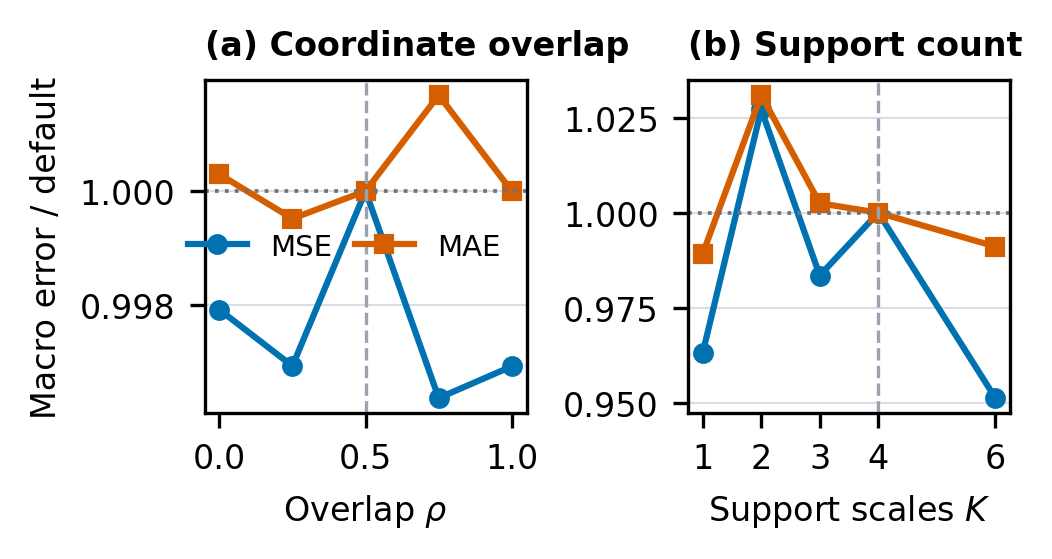
\includegraphics[width=\columnwidth]{figures/final/mesa_fig4_v675_method_sensitivity.png}
\caption{Method-parameter sensitivity on four core datasets. Validation errors
are macro-normalized by the deployed $\rho=0.5$ and $K=4$ setting.}
\label{fig:v675-method}
\end{figure}

Figure~\ref{fig:v675-method} reports one-run validation sensitivity for the
two parameters that directly control
the proposed operator: DCT-subspace overlap $\rho$ and the number of causal
support scales $K$. Varying $\rho$ over $[0,1]$ changes macro MSE/MAE by at
most $0.36\%/0.17\%$. Scale count is more
consequential: relative to $K=4$, macro deviations range from $-4.87\%$ to
$+2.71\%$ MSE and $-1.08\%$ to $+3.09\%$ MAE. No count dominates every
dataset: $K=6$ improves both metrics on HumanActivity and MHEALTH, improves
PAMAP2 MSE while slightly worsening its MAE, and does not help OPPORTUNITY,
whose best validation point is $K=3$. We therefore retain the predeclared
shared $K=4$ rather than adapting $K$ to each test dataset. Exact one-run
validation errors are reported in the supplement.

\subsection{Efficiency}

\begin{table}[t]
\centering
\setlength{\tabcolsep}{2.2pt}
\caption{Efficiency on MHEALTH (batch size 4; lower is better). Par./MACs/Mem. use M/G/GB; Tr./Inf. use ms.}
\label{tab:v665-efficiency}
\begin{tabular}{@{}lrrrrr@{}}
\toprule
Method & Par. & MACs & Mem. & Tr. & Inf. \\
\midrule
APN       & \textbf{.021} & .017 & \textbf{.043} & \textbf{5.81} & \textbf{1.30} \\
KAFNet    & .038 & \textbf{.011} & 4.425 & 10.83 & 3.41 \\
tPatchGNN & .391 & .367 & 3.121 & 81.04 & 32.42 \\
GraFITi   & .498 & 3.670 & 1.192 & 48.35 & 22.77 \\
PatchTST  & .077 & .020 & .050 & 7.27 & 1.81 \\
MESANet   & 1.733 & .305 & .151 & 23.28 & 11.24 \\
\bottomrule
\end{tabular}
\end{table}


Table~\ref{tab:v665-efficiency} compares parameter count, multiply-accumulate
operations (MACs), optimizer-step
peak memory, training latency, and inference latency on one RTX 4080. MESANet
uses 1.733M parameters and 0.305G MACs. Its
23.28-ms training step and 11.24-ms inference step are $2.08\times$ and
$2.03\times$ faster than GraFITi, while its 0.151-GB peak memory is
$7.89\times$ lower. Relative to tPatchGNN it is $3.48\times/2.89\times$
faster and uses $20.65\times$ less peak memory.
PatchTST remains the lowest-cost competitive model. MESANet therefore trades
higher cost than lightweight regular patches for lower cost than the two dense
irregular graph baselines profiled here.

\subsection{Subject and Observation-Mechanism Stress Tests}

\begin{table}[t]
\centering
\setlength{\tabcolsep}{3.0pt}
\caption{Subject-transfer and observation-mask stress results.}
\label{tab:v671-stress}
\begin{tabular}{@{}p{0.34\columnwidth}cc@{}}
\toprule
Protocol & Gain MSE/MAE & Wins MSE/MAE \\
\midrule
LOSO--MH & $+6.76/+7.08\%$ & 10/10; 10/10 \\
LOSO--USC & $+3.96/+4.19\%$ & 13/14; 14/14 \\
Group async. & $+2.98/+3.42\%$ & 3/3; 3/3 \\
Matched MCAR & $+7.78/+10.13\%$ & 3/3; 3/3 \\
Matched block & $+0.27/+2.55\%$ & 2/3; 3/3 \\
\bottomrule
\end{tabular}
\end{table}

Table~\ref{tab:v671-stress} separates two forms of distribution shift from the
main optimization-repeat benchmark. Leave-one-subject-out (LOSO) gains are
geometric means over 10
MHEALTH and 14 USC-HAD subjects; mask gains are arithmetic means over three
datasets. In strict LOSO, every test subject is
excluded from training and validation. Against the predeclared PatchTST
comparator, MESANet improves geometric MSE/MAE by $5.14\%/5.41\%$ over all 24
subjects, with 23/24 and 24/24 wins. The mean log-ratio bootstrap intervals
exclude zero on both MHEALTH and USC-HAD; fold-level errors and intervals are
reported in the supplement. This is evidence of subject transfer, not an
additional optimization-seed claim.

The one-run mask suite replaces released availability with group-asynchronous,
density-matched missing-completely-at-random (MCAR), or density-matched block
masks on MHEALTH, OPPORTUNITY, and PAMAP2. HumanActivity is excluded because
its released loader does not apply these mask-protocol controls. MESANet wins
7/9 MSE and 9/9 MAE cells. The MSE reversals are PAMAP2 under group
asynchrony ($-0.08\%$) and OPPORTUNITY under block removal ($-2.72\%$), while
MAE remains positive. The latter is a boundary under long contiguous gaps in
this run.

Across these experiments, the strongest repeated evidence concerns the frozen
main contrasts and the four-dataset component controls. LOSO measures variation
over held-out subjects with one optimization run per fold, and the mask suite
is a one-run mechanism stress test. They define transfer and missingness
boundaries rather than extend the five-run paired optimization-run comparison.

\FloatBarrier

\section{Conclusion}
We presented MESANet, an end-to-end wearable IMTS backbone that preserves an
affine-anchored multiresolution support coordinate and an ordered waveform
coordinate until bounded DCT-domain forecast formation. A validation-frozen
five-run comparison favors MESANet in mean error for 9 of 12 metric cells and
on both metrics for four datasets; six cells have paired bootstrap intervals
over optimization runs favoring MESANet. Parameter-matched controls support the dual-coordinate
factorization, multiresolution support, and ordered DCT basis, while waveform
utility is regime dependent and the controls do not show an accuracy benefit
from separate transfer parameters. The evidence supports dual-coordinate forecasting in several wearable
IMTS regimes, with HumanActivity MSE, USC-HAD, computation, and long-block
missingness remaining explicit boundaries.

\clearpage
\bibliographystyle{plainnat}
\bibliography{mesanet_references}
\end{document}
